\section{Mapping Ground View to Map Location}
The problem solved in this section can be described as follows:

Given the
continuously alternating position of a man walking around in a ground-view
image sequence, find and display his position in a top-view map.  More
generally:

Given a position in a planar projection of a space, find and display the
corresponding position in another planar projection of the same space.

\begin{figure}[h]
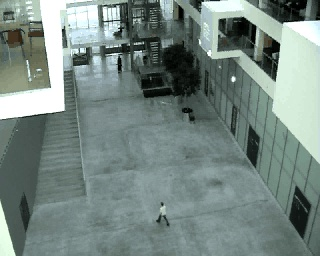
\includegraphics{./pics/Ground.jpg}
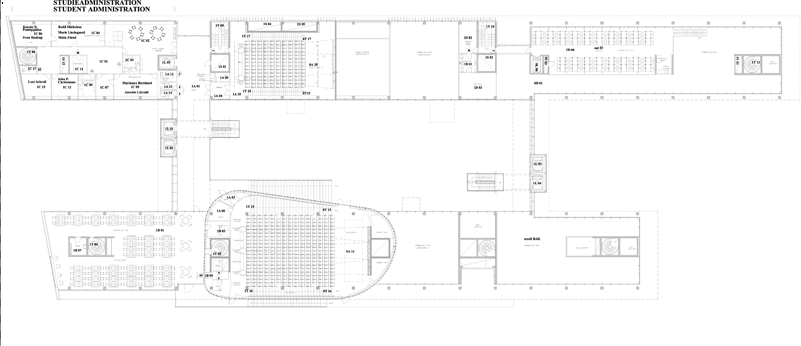
\includegraphics{./pics/ITUMap.png}
\caption{Top: Ground-view. Bottom: Top-view map}
\label{fig:groundvsmap}
\end{figure}

The ground-view image ($G$) and top-view map ($M$) are seen in figure
\ref{fig:groundvsmap}. Because they are projections of the same plane, there
exists a homography between the ground floor in $G$ and $M$. To find this
homography, the user is prompted to manually select four corresponding points
which are then inserted in a system of linear equations, the solution to which
is the homography $H_{G}^{M}$.

For each frame in the video sequence, the point $x$ in $G$ is pre multiplied
with $H_{G}^{M}$, the normalized result is the point $x'$ in $M$, that
corresponds to the mans location. $$normalize(H_{G}^{M}*x) = x'$$ The point
representing the mans location in $G$ is chosen as close to his feet as possible.
This is done because the man is \emph{not} in the same plane as $G$ floor, he
is perpendicular to it. Because of this, $H_{G}^{M}$ would transform
his head's location to a point several meters from his feet's.
